%&pdflatex
\documentclass[12pt]{article}


\usepackage{graphicx}
\graphicspath{ {images/} }
\usepackage{colortbl}
\usepackage{xr}
\usepackage{longtable}
\usepackage{xfrac}
\usepackage{tabularx}
\usepackage{booktabs}
\usepackage{hyperref}
\usepackage{xcolor} % for different colour comments
\usepackage{fullpage}
\newcounter{rowcount}
\setcounter{rowcount}{0}
\usepackage{tikz}
\usetikzlibrary{shapes,arrows}


%% Diagram formatting
\tikzstyle{block} = [draw, rectangle, minimum height=1.5em, minimum
width=2em, text centered]
\tikzstyle{arrow} = [thick,-,>=stealth]


\hypersetup{
    bookmarks=true,         % show bookmarks bar?
    colorlinks=true,        % false: boxed links; true: colored links
    linkcolor=blue,        % color of internal links (change box color with linkbordercolor)
    citecolor=green,        % color of links to bibliography
    filecolor=magenta,      % color of file links
    urlcolor=cyan           % color of external links
}

%% Comments
\newif\ifcomments\commentstrue
\ifcomments
\newcommand{\authornote}[3]{\textcolor{#1}{[#3 ---#2]}}
\newcommand{\todo}[1]{\textcolor{red}{[TODO: #1]}}
\else
\newcommand{\authornote}[3]{}
\newcommand{\todo}[1]{}
\fi
\newcommand{\wss}[1]{\authornote{magenta}{SS}{#1}}
\newcommand{\ds}[1]{\authornote{blue}{DS}{#1}}
\newcommand{\kly}[1]{\authornote{green}{KL}{#1}}
\newcommand{\cc}[1]{\authornote{orange}{CC}{#1}}

%%%%%%%%%%%%%%%%%%%%%%%%%%%%%

\begin{document}

\title{User Manual}
\author{Team 6\\ \\James Anthony (anthonjb)\\ Wenqiang Chen (chenw25)\\ Carolyn Chong
(chongce)\\ Kevin Ly (lyk2)}
\date{\today}

\maketitle

\pagebreak

\tableofcontents
\listoffigures

\section*{Revision History}
\begin{tabular}{|c|c|}
\hline
\textbf{Date}  & \textbf{Comments} \\ \hline
February 28, 2016 & Revision 0 \\ \hline
\end{tabular}

\pagebreak

%%%%%%%%%%%%%%%%%%%%%%%%%%%%%

%%%%%%%%%%%%%%%%%%%%%%%%%%%%%% Introduction
\section{Introduction}

Words

%%%%%%%%%%%%%%%%%%%%%%%%%%%%%% Copyright
\section{Copyright}

%%%%%%%%%%%%%%%%%%%%%%%%%%%%%% About this Manual
\section{About this Manual}

%%%%%%%%%%%%%%%%%%%%%%%%%%%%%%
\section{Installation}

%%%%%%%%%%%%%%%%%%%%%%%%%%%%%% Tasks
\section{Tasks}

\subsection{Registration}
\label{sec:registration}
All user must have a registered account before using Quarters. Registration process is simple and easy, only a valid email and a password is required.\\\\
You can create an account by following these instructions:

\begin{enumerate}
    \item Click on "SIGN UP" button on the top of the homepage, or Click on "LOGIN" button then select "Register" tab
    \item Enter a valid email address and password
    \item Click on "REGISTER NOW"
    \item An email will be sent to the specified email address, which will contain a link for you to activate your account.
\end{enumerate}
\subsection{Login}
All user must be logged in to use any of the Quarters' features. If you do you have an account, please refer to \hyperref[sec:registration]{Registration} to create an account. \\ \\
You can login by following these instructions:
\begin{enumerate}
    \item Click on "LOGIN" on the top of the homepage, or Click on "SIGN UP" button and switch to "Login" tab
    \item Enter your registered email address and password
    \item Click on "LOG IN"
\end{enumerate}
\subsection{House Management}

\subsection{User Profile}

\subsection{House Information}

\subsection{Document Upload}

\subsection{Bulletin Board}

\subsection{Finance}

\subsection{Maintenance}
To access the Maintenance page, click on "Maintenance" under the navigation bar. The Maintenance page displays a list of all the maintenance tickets created in the house in chronological order. It  allows a user to send maintenance requests to another user for them to address and resolve. Any user can send a request to any user in the same house. Each request has a priority level assigned to it to inform the receiver of the urgency of a response. Figure \ref{fig:maintenance} shows a screen image of the Maintenance page.

\begin{figure}
\centering
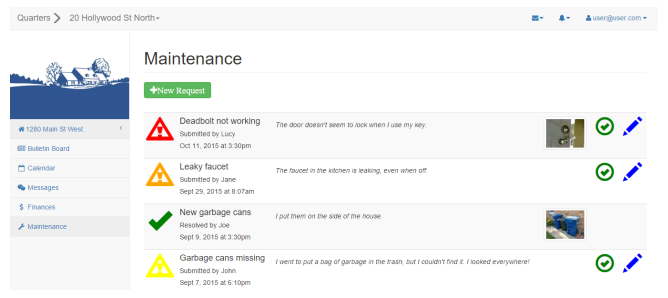
\includegraphics[width=\textwidth]{maintenance}
\caption{Screen image of Maintenance page}
\label{fig:maintenance}
\end{figure}

\subsubsection{Add a Ticket}
\begin{enumerate}
\item To add a ticket, click on the "New Request" button' at the top of the Maintenance page. A pop-up modal will appear with fields for user input.
\item Fill out the fields. Note: All fields marked with an asterisk (*) must be filled.
\item Click the "Submit" button at the bottom of the modal. The modal will close.
\item The new request will display at the top of the Maintenance page above all of the other tickets.
\end{enumerate}

\subsubsection{Edit a Ticket}
Only the creator of a ticket can edit the same ticket.
\begin{enumerate}
\item To edit a ticket, click on the blue pencil to the right of the relevant ticket. A pop-up modal will appear with editable fields.
\item Edit the appropriate fields.
\item Click on the "Submit" button at the bottom of the modal. The modal will close.
\item The updated ticket will display in its original ordering.
\end{enumerate}

\subsubsection{Delete a Ticket}
Only the creator of a ticket can delete the same ticket.
\begin{enumerate}
\item To delete a ticket, click on the red "X" to the right of the relevant ticket. A confirm modal will appear.
\item Click "OK" to delete the ticket. The modal will close.
\item The deleted ticket will no longer be displayed.
\end{enumerate}

\subsubsection{Resolve a Ticket}
Only the receiver of a ticket can resolve the same ticket.
\begin{enumerate}
\item To resolve a ticket, click on the green checkmark to the right of the relevant ticket. A confirm modal will appear.
\item Click "OK". The modal will close.
\item The resolved ticket will display at the top of the Maintenance page above all of the other tickets. A green checkmark will replace the priority level symbol that was originally displayed on the left of the ticket.
\end{enumerate}


\subsection{Calendar}
To access the Calendar page, click on "Calendar" under the navigation bar. The Calendar page displays a calendar showing all events created by members of the same house. Any user can add an event to the house's calendar. Figure \ref{fig:calendar} shows a screen image of the Calendar page.

\begin{figure}
\centering
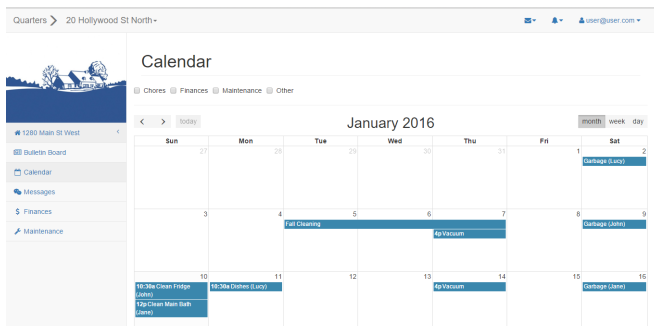
\includegraphics[width=\textwidth]{calendar}
\caption{Screen image of Calendar page}
\label{fig:calendar}
\end{figure}

\subsubsection{Change Calendar View}
\begin{enumerate}
\item The default calendar view is monthly. To change the calendar view, above the calendar, to the right, click the "Month" or "Week" or "Day" button. The calendar view will change.
\end{enumerate}

\subsubsection{Move Forward or Backward}
\begin{enumerate}
\item To move the calendar forward to the next month/week/day,  above the calendar, to the left, click the "$>$" button.
\item To move the calendar backward to the previous month/week/day,  above the calendar, to the left, click the "$<$" button.
\end{enumerate}

\subsubsection{Add an Event}
To add an event to the calendar, there are two methods: \\
Method 1:
\begin{enumerate}
\item Navigate to the desired day (and time if in week or day view).
\item Click on the desired day (and time if in week or day view). A pop-up modal will appear with fields for user input.
\item Fill out the fields. Note: All fields marked with an asterisk (*) must be filled.
\item Click the "Submit" button at the bottom of the modal. The modal will close.
\item The new event will display on the calendar.
\end{enumerate}
Method 2:
\begin{enumerate}
\item Click on the "New Event" button at the top of the Calendar page. A pop-up modal will appear with fields for user input.
\item Fill out the fields. Note: All fields marked with an asterisk (*) must be filled.
\item Click the "Submit" button at the bottom of the modal. The modal will close.
\item The new event will display on the calendar.
\end{enumerate}

\subsubsection{Edit an Event}
Only the creator of an event can edit the same event.
\begin{enumerate}
\item To edit an event, navigate to the desired event on the calendar.
\item Click on the desired event. A pop-up modal will appear with editable fields.
\item Edit the appropriate fields.
\item Click on the "Submit" button at the bottom of the modal. The modal will close.
\item The updated event will display on the calendar.
\end{enumerate}

\subsubsection{Delete an Event}
Only the creator of an event can delete the same event.
\begin{enumerate}
\item To delete an event, navigate to the desired event on the calendar.
\item Click on the desired event. A pop-up modal will appear.
\item Click on the "Delete" button beside the "Submit" button at the bottom of the modal.  A confirm modal will appear.
\item Click "OK" to delete the event. The modals will close.
\item The deleted event will no longer be displayed on the calendar.
\end{enumerate}

\subsection{Notifications}



%%%%%%%%%%%%%%%%%%%%%%%%%%%%%% Troubleshooting
\section{Troubleshooting}

%%%%%%%%%%%%%%%%%%%%%%%%%%%%%% Frequently Asked Questions
\section{Frequently Asked Questions}

%%%%%%%%%%%%%%%%%%%%%%%%%%%%%% Safety and Precautions

\end{document}
